\section{Discussion}

\subsubsection{Correspondence search}

KLT vs Harris matching
\textcolor[rgb]{1,0,0}{@ Milan}

\subsubsection{Bundle-adjustment}
improvements reached
\textcolor[rgb]{1,0,0}{@Miro}

\subsubsection{Pose estimation algorithm}
We investigated pose estimation with DLT refinement after the P3P-Guess and without refinement (using the last P3P guess from RANSAC). It turned out, that very often the P3P-guess was a lot better and especially more robust then the DLT refinement. \cref{parking_result_fig_dlt} shows the estimated trajectory with DLT refinement. It is clearly worse then the P3P estimate as shown in \cref{parking_result_fig}. That's why we used the last P3P guess in our implementation.
\begin{figure*}[ht!]
    \centering
    \begin{subfigure}[t]{0.5\textwidth}
        \centering
        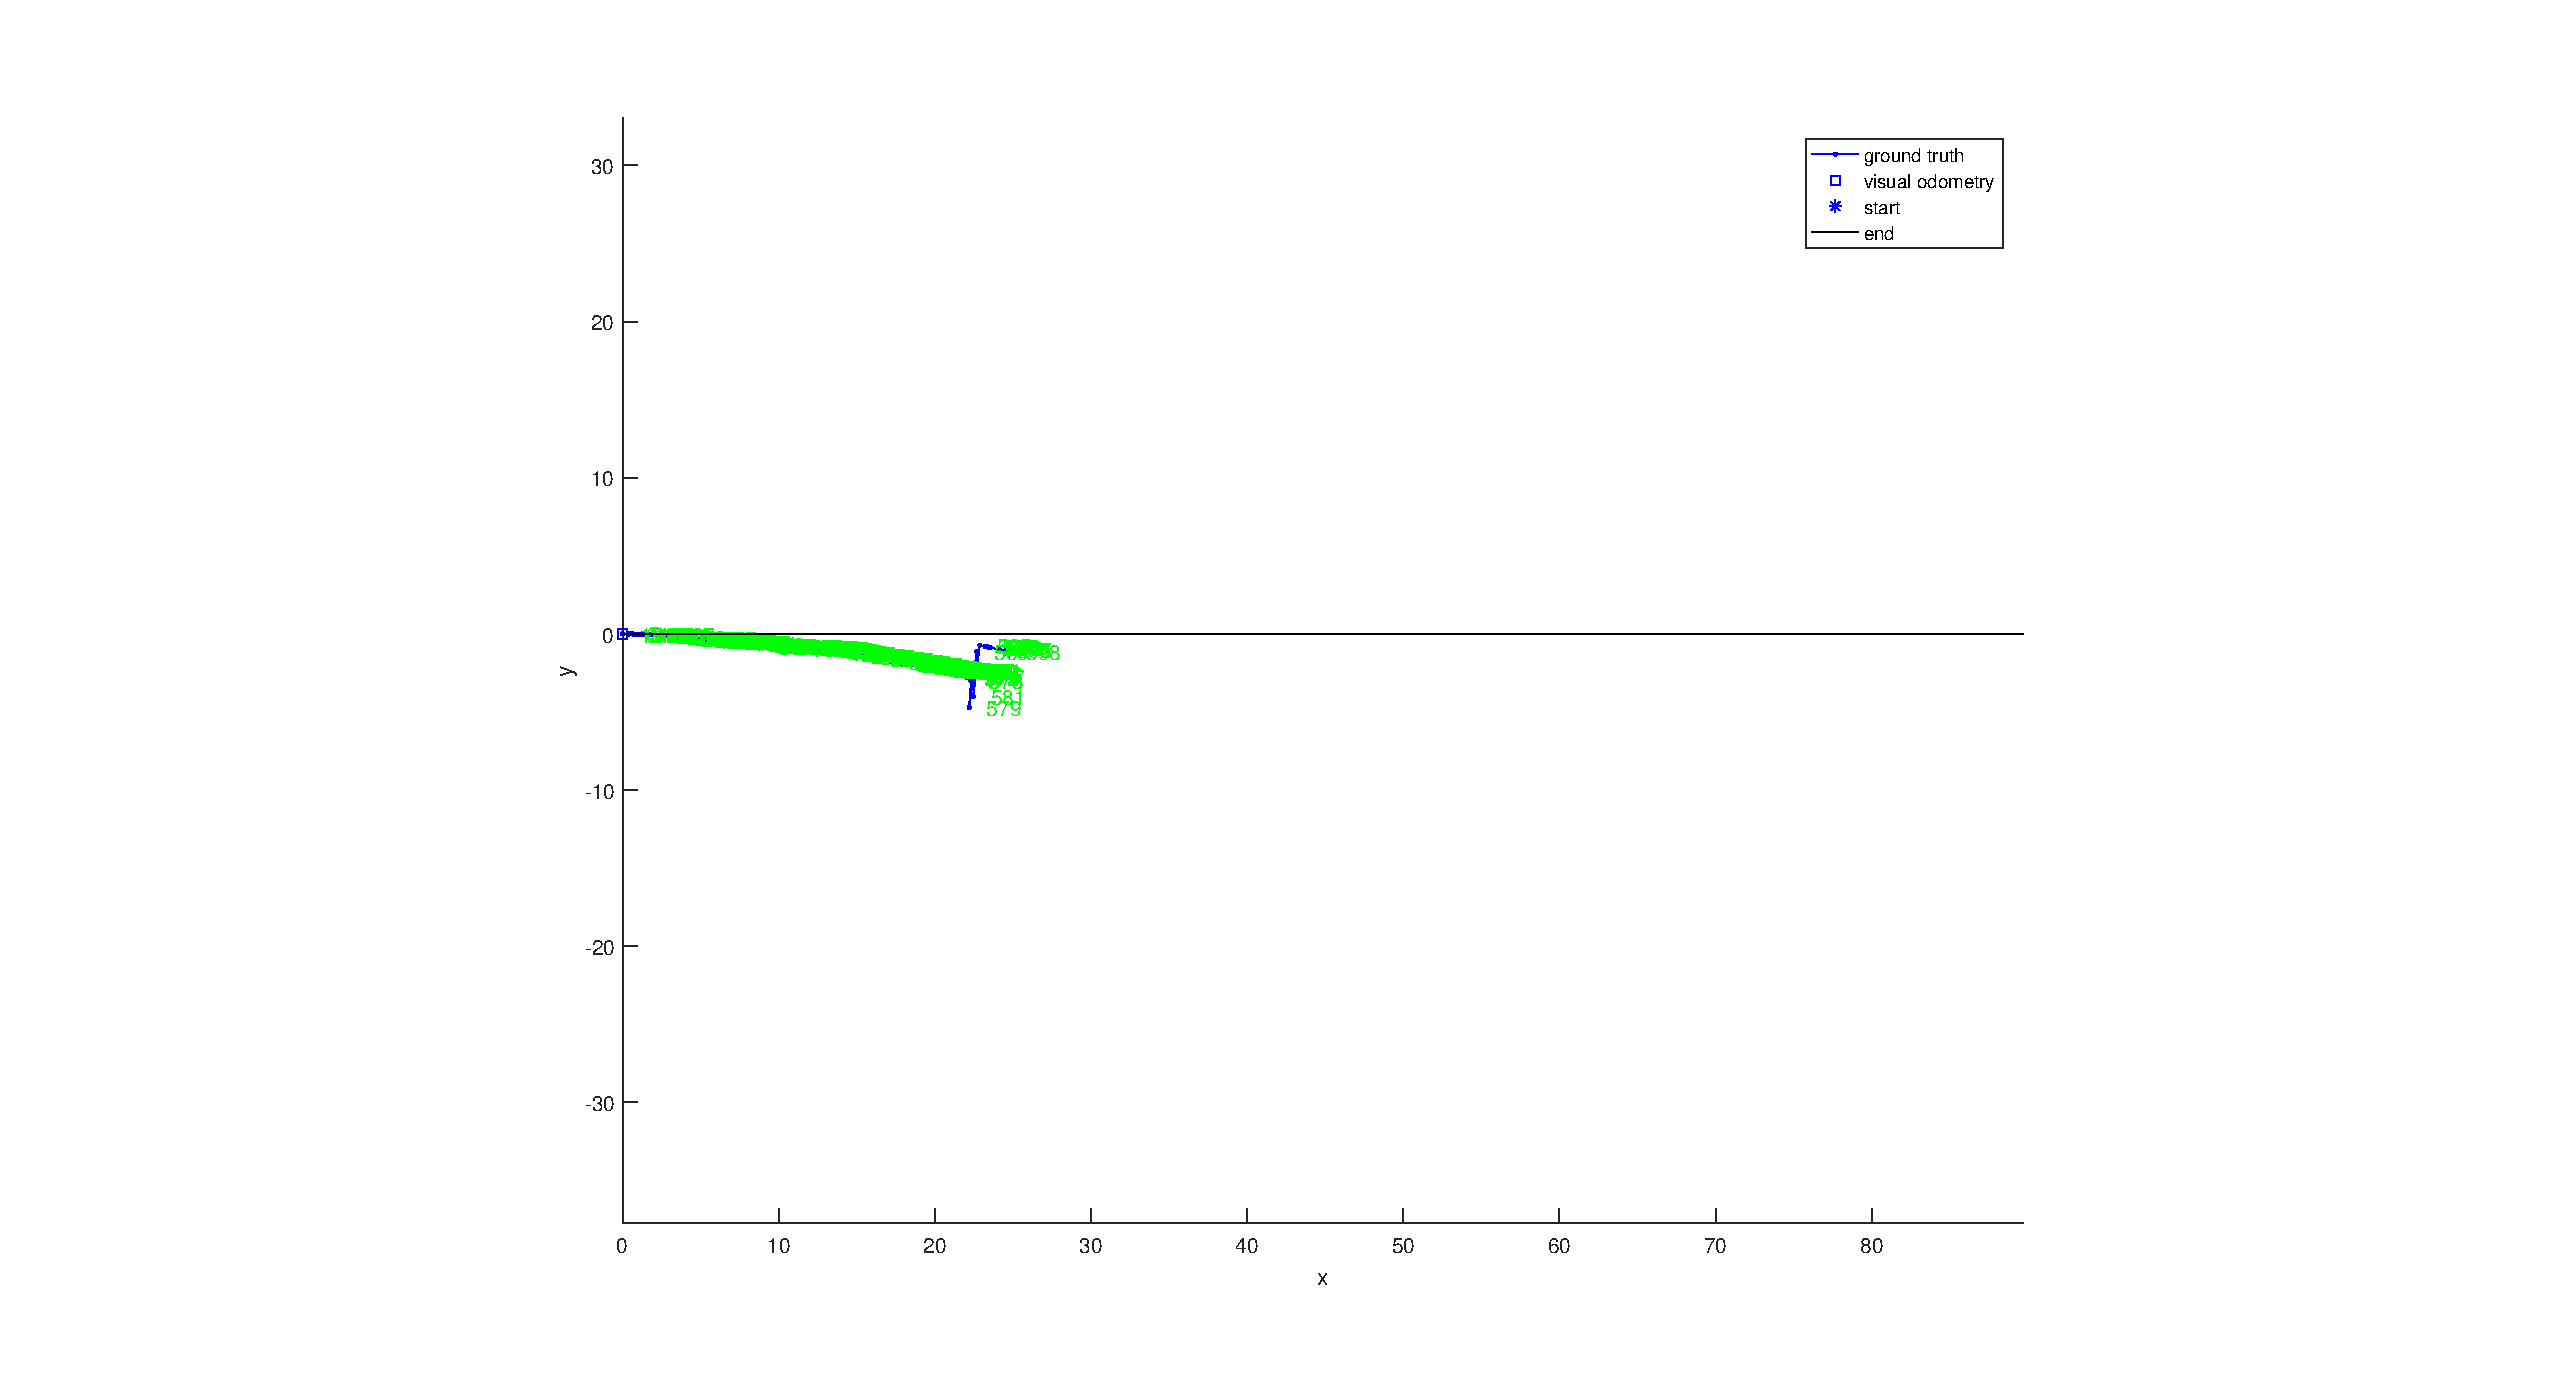
\includegraphics[height=2.7in]{results/trajectory_parking_dlt.eps} 
        \caption{Trajectory vs. ground truth}
    \end{subfigure}%
    ~ 
    \begin{subfigure}[t]{0.5\textwidth}
        \centering
        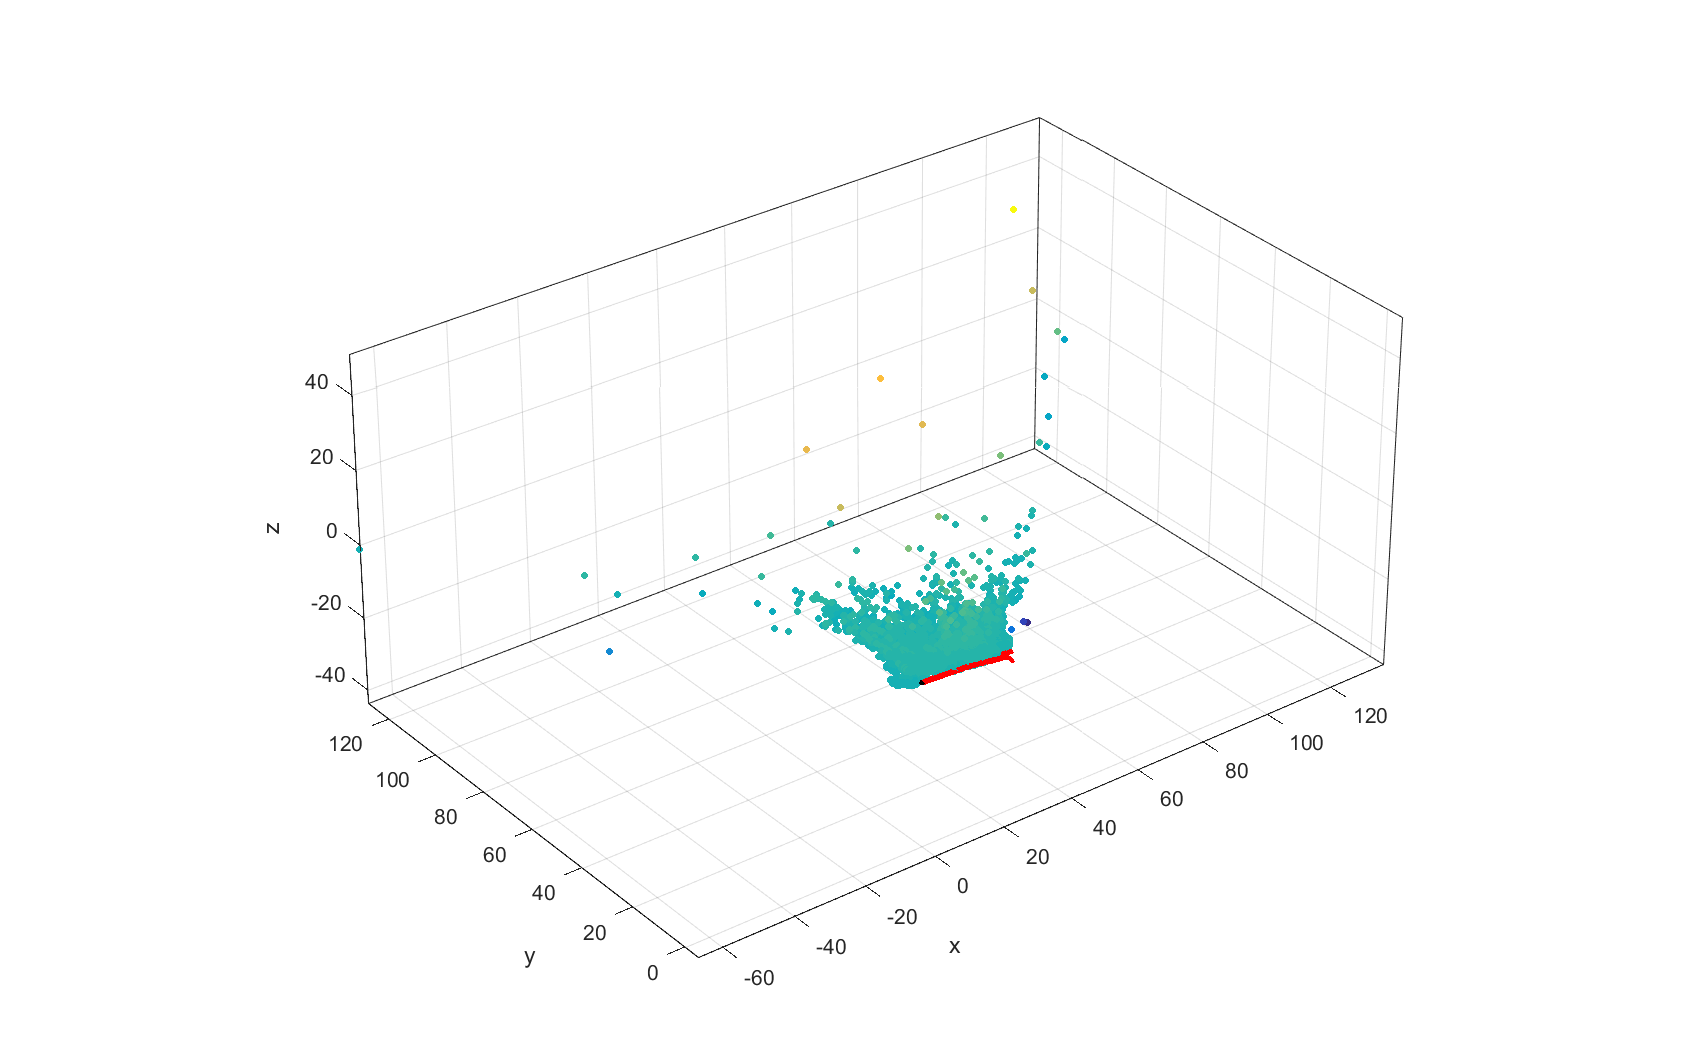
\includegraphics[height=2.7in]{results/landmarks_parking_dlt.eps}
        \caption{3D landmarks}
    \end{subfigure}
    \caption{Parking dataset results with DLT refinement}
		\label{parking_result_fig_dlt}
\end{figure*}

\subsubsection{Reinitialization}
The Reinitialization prevents the pipeline from dying of a lack of landmarks. I. E. if there are too few landmarks left, the reinitialisation interrupts the keypoint tracker and generates new landmarks. How often this happens depends on the parameters mentioned in \cref{sec_key_params} as well as on the dataset. The pipeline loses keypoints when areas with a high keypoint density are moving out of the image quickly. We could observe a small buckle of the trajectory every time the reinitialization was done.


\subsubsection{Feature work}
A list of potential improvements
\textcolor[rgb]{1,0,0}{@ Milan}

Possible future work, improvements (loop closure, ...)

\begin{itemize}
\item \colorbox[rgb]{1,0,0}{bootstrapping with both information rotation through bearing angle diff and translation through baseline/depth ratio}
\item Include bundle adjustment
\item Optimize runtime e.g. use a parallel for loop for P3P-RANSAC
\item Reinitialize depending on $T_{C_iC_j}$ instead of number of landmarks remaining. An unusually big translation or rotation $T_{C_iC_j}$ is a sign that the pipeline start diverging.
\item Loop closure and place recognition (e.g. with bag of words approach).
\end{itemize}
